% HW Template for CS 6150, taken from https://www.cs.cmu.edu/~ckingsf/class/02-714/hw-template.tex
%
% You don't need to use LaTeX or this template, but you must turn your homework in as
% a typeset PDF somehow.
%
% How to use:
%    1. Update your information in section "A" below
%    2. Write your answers in section "B" below. Precede answers for all 
%       parts of a question with the command "\question{n}{desc}" where n is
%       the question number and "desc" is a short, one-line description of 
%       the problem. There is no need to restate the problem.
%    3. If a question has multiple parts, precede the answer to part x with the
%       command "\part{x}".
%    4. If a problem asks you to design an algorithm, use the commands
%       \algorithm, \correctness, \runtime to precede your discussion of the 
%       description of the algorithm, its correctness, and its running time, respectively.
%    5. You can include graphics by using the command \includegraphics{FILENAME}
%
\documentclass[11pt]{article}
\usepackage{amsmath,amssymb,amsthm}
\usepackage{graphicx}
\usepackage[margin=1in]{geometry}
\usepackage{fancyhdr}
\usepackage{tabu}
\usepackage{framed}
\usepackage{algorithm}
\usepackage{algpseudocode}
\usepackage{pifont}
\setlength{\parindent}{0pt}
\setlength{\parskip}{5pt plus 1pt}
\setlength{\headheight}{13.6pt}
\newcommand\question[2]{\vspace{.25in}\hrule\textbf{#1}\vspace{.5em}\hrule\vspace{.10in}}
\renewcommand\part[1]{\vspace{.10in}\textbf{(#1)}}
\newcommand\algorith{\vspace{.10in}\textbf{Algorithm: }}
\newcommand\correctness{\vspace{.10in}\textbf{Correctness: }}
\newcommand\runtime{\vspace{.10in}\textbf{Running time: }}
\pagestyle{fancyplain}
\lhead{\textbf{\NAME\ (\UID)}}
\chead{\textbf{HW\HWNUM}}
\rhead{CS 6490, \today}
\begin{document}\raggedright
%Section A==============Change the values below to match your information==================
\newcommand\NAME{Jake Pitkin}  % your name
\newcommand\UID{u0891770}     % your utah UID
\newcommand\HWNUM{5}              % the homework number
%Section B==============Put your answers to the questions below here=======================

\question{Question 1}

\part{a} \textbf{Is it possible to encapsulate an AH packet within an ESP packet and vice versa? Explain with the help of examples.}

Consider the scenario (similar to Figure 17-3 in the text) where Alice and Bob are using IPsec and two firewalls, F1 and F2, between them are also using IPsec.

First, the scenario where the firewalls are using AH packets and Alice/Bob are using ESP packets, both using tunnel mode.

\begin{figure}[H]
  \centerline{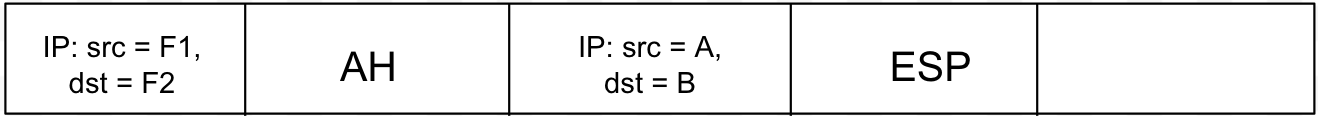
\includegraphics[width=0.5\linewidth]{hw5_1b_1.png}}
\end{figure}

This scenario does \textbf{not} work. One difference of the integrity protection provided by AH/ESP is that AH provides integrity protection of the IP header. The IPsec between F1 and F2 cannot perform the integrity protection of Alice and Bob's IP header as it is inside an encrypted ESP packet and the F1/F2 do not have the key.

To get this scenario to work, Alice and Bob need to use transport mode. In transport mode the original IP header is not encrypted. This allows AH to perform it's integrity protection of the IP header.

Alternatively, the firewalls could be using ESP packets and Alice/Bob are using AH packets.

\begin{figure}[H]
  \centerline{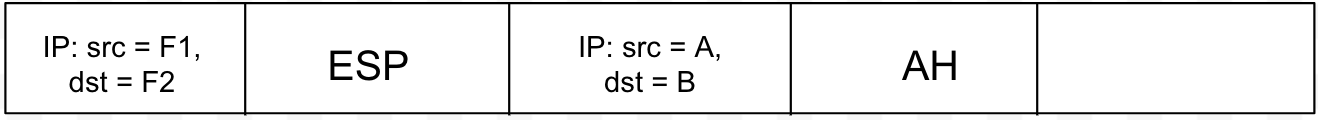
\includegraphics[width=0.5\linewidth]{hw5_1b_2.png}}
\end{figure}

In this scenario, the encapsulation of an AH packet inside a ESP packet \textbf{will} work. The IPsec between the routers are using ESP and do not check the IP headers during the integrity process.


\part{b} \textbf{Suppose Alice is sending packets to Bob using IPsec. Suppose Bob's TCP acknowledgement gets lost, and Alice's TCP, assuming the packet was lost, retransmits the packet. Will Bob's IPsec implementation notice that the packet is a duplicate and discard it?}

Bob's IPsec implementation will \textbf{not} notice it as a duplicate packet. Both AH and ESP IPsec headers have a \textit{sequence number} field that function identically. This sequence number is used by IPsec to prevent replay attacks.

TCP handles the retransmission of packets. When TCP retransmits a packet, AH/ESP will treat it as a new packet with a new sequence number. This is one of the pros of building IPsec on top of TCP: it can hand-off the responsibility of guaranteed delivery (and discarding duplicate packets).

\part{d} \textbf{Why is IPsec not firewall-friendly?}

A firewall looks at the fields in the transport layer (such as port and protocol) as part of its filtering process. Using the ESP protocol with IPsec encrypts this information and the firewall does not have the ability to decrypt this information. Solutions include terminating IPsec at the firewall or trusting the endpoint and forwarding the encrypted packet to the endpoint.

\question{Question 2}

\part{a} \textbf{Why does the HMAC computation in SSL data transfer phase use a sequence number with each record even though SSL is built on top of TCP that delivers data in the correct order?}

During the transfer phase of SSL, HMAC is used for integrity protection of the message. Part of the data that is hashed is a sequence number. This sequence number is never actually transmitted as SSL is built on top of TCP which handles in-order delivery. 

This sequence number is kept as state and is used to \textbf{protect against reply/ordering attacks}. If TCP manages to fail (or someone is being malicious) and the packets do not not arrive in order, the HMAC will detect this.

\part{b} \textbf{This question pertains to 3G-UMTS security. Consider the case when a user visits another country and turns her phone on to make a phone call and notices service X. However, it is possble that service provider X is actually service provider Y that charges a lot more for phone calls made while roaming. The service provider Y when working as the intermediary between the subscriber and the user's home network appears to be X to the user by stays as Y for the home network. How does the home network ensure that the user knows the service provider it is actually connecting to?}



\part{c} \textbf{What are two advantages of computing the response to the challenge in the SIM card for GSM authentication?}

\textit{Advantage 1:} The SIM card is unique to the user and contains their subscription information. By containing this all in the SIM card, it makes it easy for the user to switch the SIM card to another device and still use the same secret key for authentication. The user doesn't have to trust mobile device creators and only have to trust their wireless provider.

\textit{Advantage 2:} The A3 and A8 algorithms run inside the SIM card to respond to challenges. These algorithms could be changed (updated to be more secure) by the Home Network (HLR) by making changes on their end and on the SIM card. This is an advantage as it is rare that a protocol or algorithm can be updated this easily.


\part{d} \textbf{What are two problems in deploying DDoS prevention solutions close to the sources of attack traffic?}

\textit{Problem 1:} A DDoS attack is made possible by a distributed collection of computers targeting a server. It's common for these computers to be compromised devices that are now used as attack agents. A good prevention solution to DDoS attacks would be to increase the security of these devices so they can't be used as attack agents. Sadly there is little motivation for this to happen as the compromised computers are rarely affected. Lack of motivation is a common theme of cause for security vulneriabilies.

\textit{Problem 2:} A second problem is the inherent structure of how the Internet is designed. Packets are routed to a destination address by routers. These routers are not concerned with security issues, the security and handling of packets is delegated to the destination machine (and the source machine but we have seen there is little motivation on their end to stop DDoS attacks). As such, we would have to redesign crucial parts of the Internet stack such as routing if we wanted to tackle DDoS attacks not on the targeted server (and close to the sources of attack).

\part{e} \textbf{Could the Local Aggregate Congestion Control mechanism for DDoS prevention result in collateral damage? Explain your answer.}

Yes the Local Aggregate Congestion Control mechanism can result in collateral damage. During this mechanism, a router detects when it's dropping a large number of packets. The offending packets are aggregated together and their rate is severely limited. Now no system is perfect and legitimate traffic will be aggregated with malicious traffic. As a result a genuine user's rate will become limited.

\part{f} \textbf{Would it make sense to use crypto cookies in conjunction with IP traceback? Explain briefly.}

Both could be used as two layers of defense against DDoS attacks, but they are separate approaches. A downside I could see of this is there would be too much collateral damage as a genuine user doubles their chance of their rate unintentionally being throttled or blocked.

\part{g} \textbf{What is a bloom filter? How could it be used to filter IP packets?}

A bloom filter is a set that uses probability to make it space efficient. It consists of an array of m bits and K independent hash functions and represents a set A that contains n elements. Each of the n elements is hashed by the K functions and the ouputs are positions of the m-bit vector. Given a new incoming element b, we can apply the hash functions to b and see if it produces 1's in all the bit positions. If it does, then it is an element of A. The catch is there is a (small) probabilistic chance of a false positive. That is, we say b belongs to A when it doesn't.

This can be used to filter IP packets. Let A be a collection of problematic IP addresses. As a new address b comes in, we can see if it belongs to A and filter it out. There runs a small chance that we label a non-malicious IP address as malicious.

\part{h} \textbf{Why doesn't the Botz-for-sale system use only one TCP connection to send the puzzle and receive the response instead of using two TCP connections?}

When the Botz-for-sale system sends the puzzle, it protects itself from DDoS attacks related to using the TCP handshake phase to overload a system. Kill-Bots provides a modification to the TCP stack on the server and it sends the puzzle in a 1-2 packet at the end of the TCP handshake. This prevents maintaining any connection state so the server can't be overwhelmed by a distributed attack of handshake messages. Since no state is kept, a second TCP connection is required to get the response.

\part{i} \textbf{Why does it make sense to use an onion that encrypts information using public keys in the connection set up phase but secret keys during data movement?}

It makes sense to use public keys during the connection set up as the end point is connecting to an onion proxy. An onion proxy is a trusted node and knows the true source and destination address of the packets being transmitted.

During the data transmission step, there are multiple layers of encryption. This is essential to maintaining anonymity and keys must be secret. If they weren't, someone who wants to trace your identity could do so. 


\question{Question 3}

\part{1} \textbf{What are the advantages of building security at the TCP layer?}

There are many advantages to building security at the TCP layer. Since TCPsec is built on top of TCP, it can take advantage of some of the features of TCP. TCPsec can use TCP's guarantee of in-order delivery. Additionally it can use TCP's handshake phase to exchange keys used for TCPsec, removing an extra handshake phase. 

By moving security to the transport layer, it provides end-to-end security. Maybe applications already use TCP and can update their kernel and set the TCP flags for quick deployment.

\part{2} \textbf{What flexibility does TCPsec provide for encrypting the TCP segment?}

Similar to SSL, TCPsec provides flexibility to the user for how to encrypt the TCP segment. First, encryption and integrity protection are independent operations and can be done in any order. Second, the user can specify which crypto algorithms they would like to be used for these operations. As for the actual encryption, the TCP payload is always encrypted. TCPsec leaves the option up to the user to encrypt portions of the IP header as well. 

\part{3} \textbf{How does TCPsec interoperate with NATS?}

During the TCPsec handshake, a NAT option is provided. To detect if there are NATS (aka there are NATS on the path to the destination) the first SYN message is used. The NAT option contains the source IP address and port numbers. TCPsec can detect if these are changed (by a NAT) along the path to the destination. If detected, these new values can be used during message digest integrity checks and TCPsec plays well with NATS.

\part{4} \textbf{Why does TCPsec handshake perform better than SSL?}

SSL is deployed at the application layer. To perform an SSL handshake, a TCP connection is opened and the SSL handshake is performed over this connection. This TCP connection needs to perform the typical 3-way handshake to establish the connection. Once established, the application can use this connection to perform the SSL handshake, which requires multiple TCP packets to be transmitted back and forth.

In TCPsec, the security handshake is performed at the same time as the TCPsec 4-way handshake (a modified version of the 3-way TCP handshake). As you could imagine, this will be more performant than the SSL handshake.

\end{document}